\newpage
\chapter{Комуникация клиент-сървър}
\label{chapter06}

Комуникацията между Android клиента и PHP базирания сървър се извършва през HTTP с размяна на JSON пакетирани съобщения. 

\section{Hypertext Transfer Protocol}

При всяко създаване на инстанция за тапета е нужно да се извърши свързване към отдалечения сървър и да бъде заявен пакет за работа. Ако връзката не е възможна се използват данните, записани в локалната база данни. 

\begin{figure}[h]
  \centering
  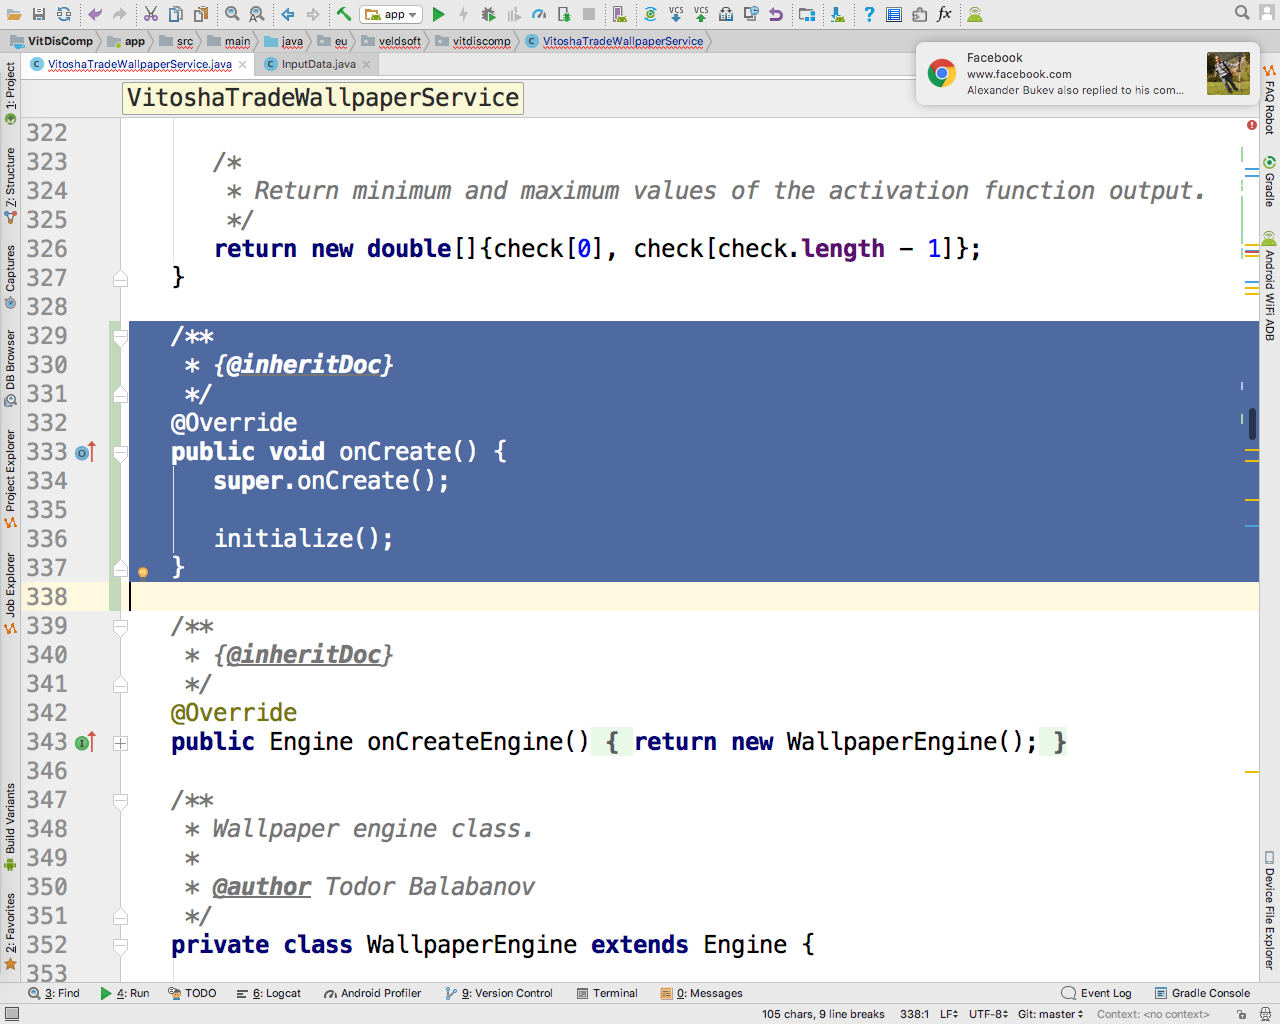
\includegraphics[height=0.45\pdfpageheight]{pic0155}
  \caption{Инициализация на вътрешните променливи}
\label{fig:pic0155}
\end{figure}
\FloatBarrier

Инициализацията на вътрешните променливи се осъществява в събитието onCreate (Фиг. \ref{fig:pic0155}).

\begin{figure}[h]
  \centering
  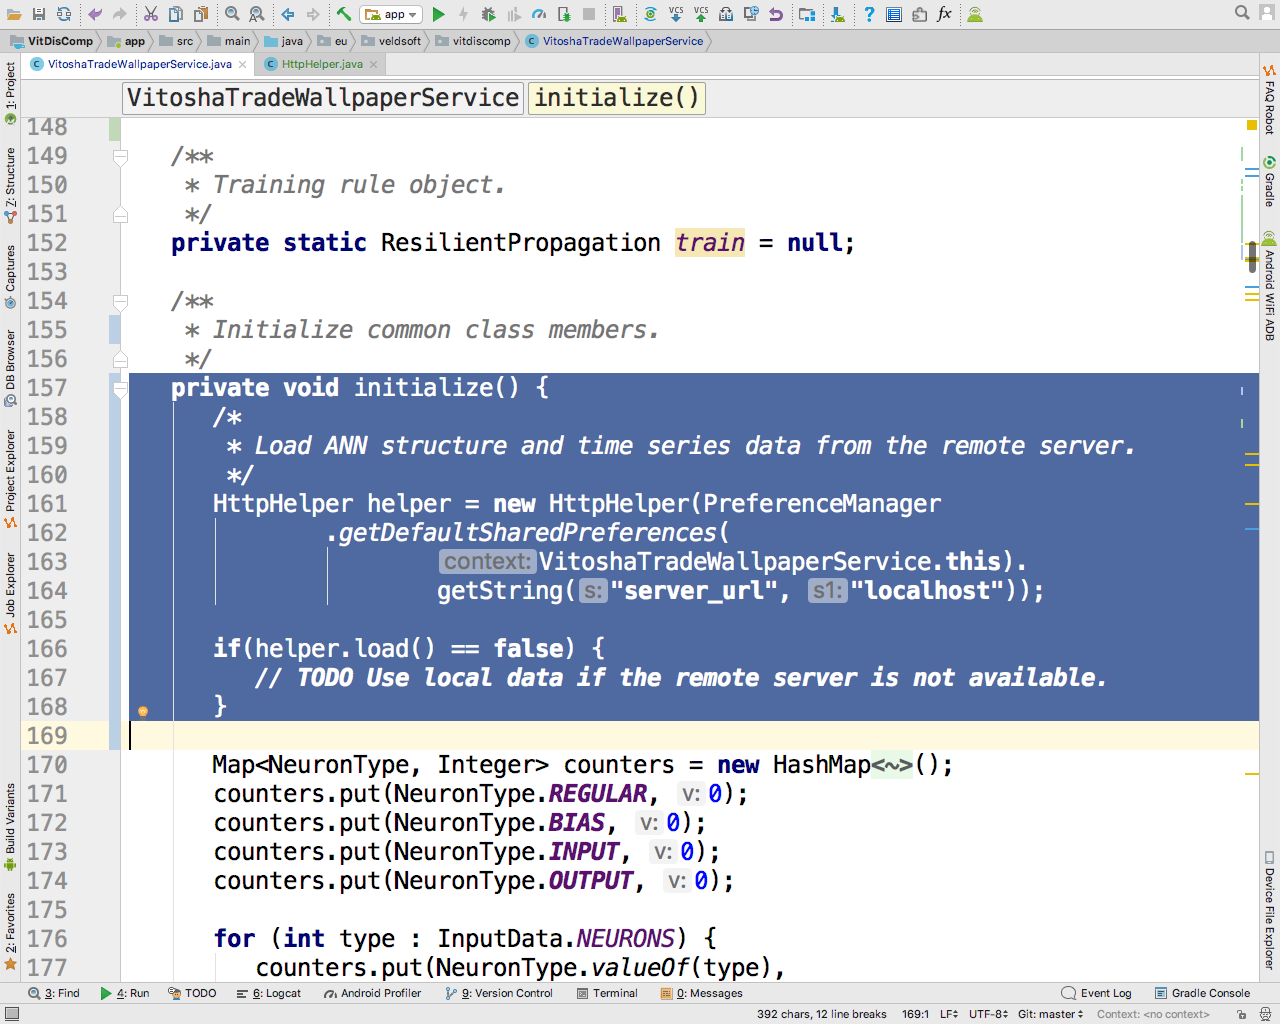
\includegraphics[height=0.45\pdfpageheight]{pic0156}
  \caption{Зареждане на данните с помощта на HTTP комуникация}
\label{fig:pic0156}
\end{figure}
\FloatBarrier

Инициализирането на вътрешните променливи през HTTP се поема от допълнително създаден помощен обект, който е от клас отговорен за комуникацията (Фиг. \ref{fig:pic0156}). 

\begin{figure}[h]
  \centering
  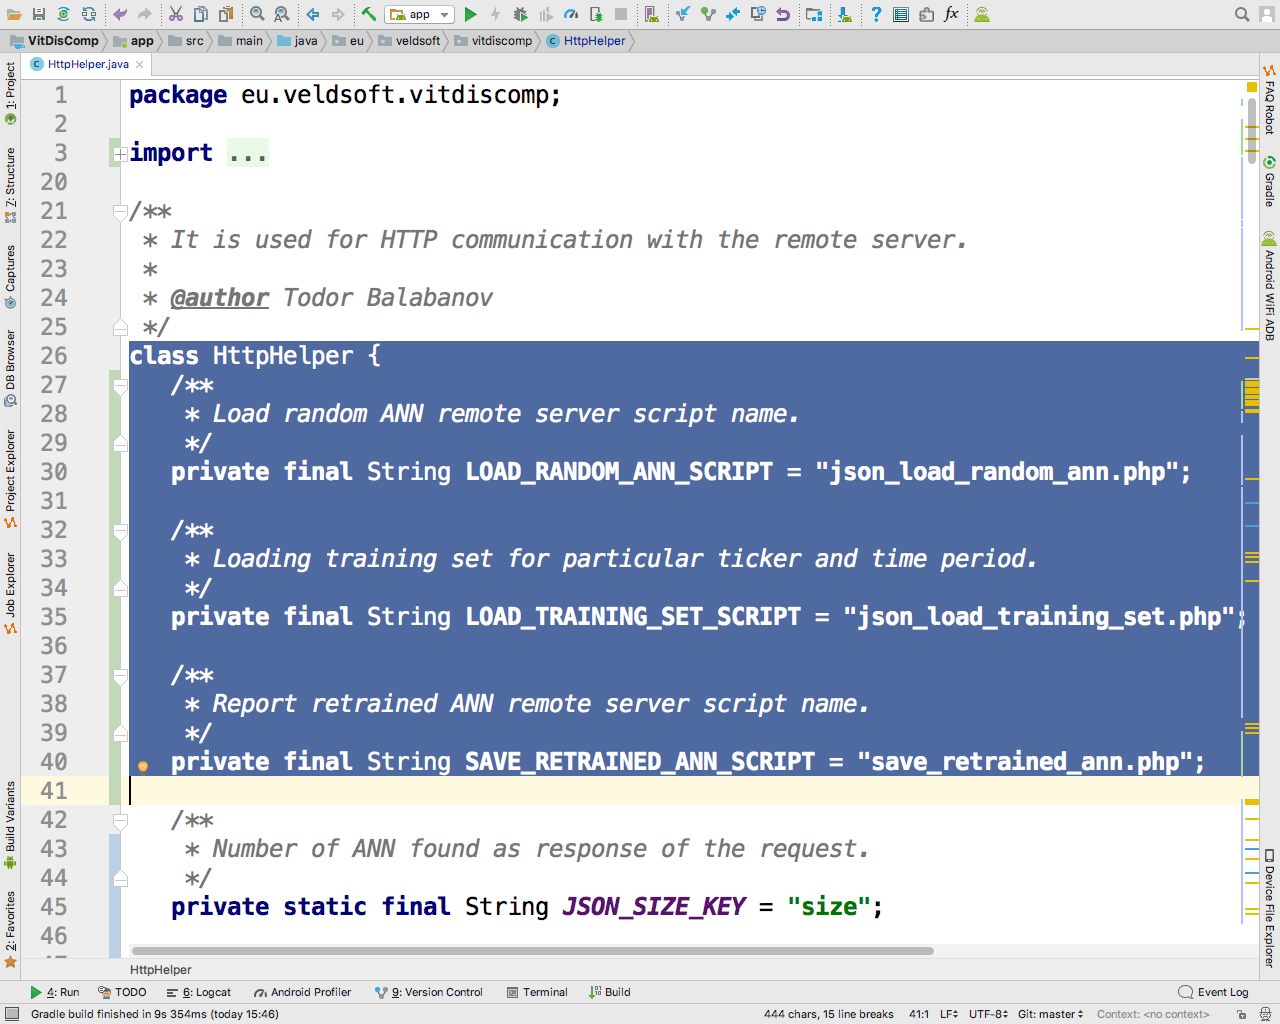
\includegraphics[height=0.45\pdfpageheight]{pic0159}
  \caption{HTTP комуникационен файл}
\label{fig:pic0159}
\end{figure}
\FloatBarrier

Комуникацията  по HTTP с отдалечения сървър и синтактичната обработка на JSON съобщенията са изнесени в помощен клас HttpHelper (Фиг. \ref{fig:pic0159}). Съществуват различни възможности за задаване на имената, които се ползват за отдалечените скриптове, но един от най-елементарните е чрез именувани константи. Имената на сървърните скриптове подлежат на промяна, но се разчита, че тя ще е значително по-рядко от смяната на URL адреса. Точно поради тази причина параметризирането на информацията е по различен начин. 

\begin{figure}[h]
  \centering
  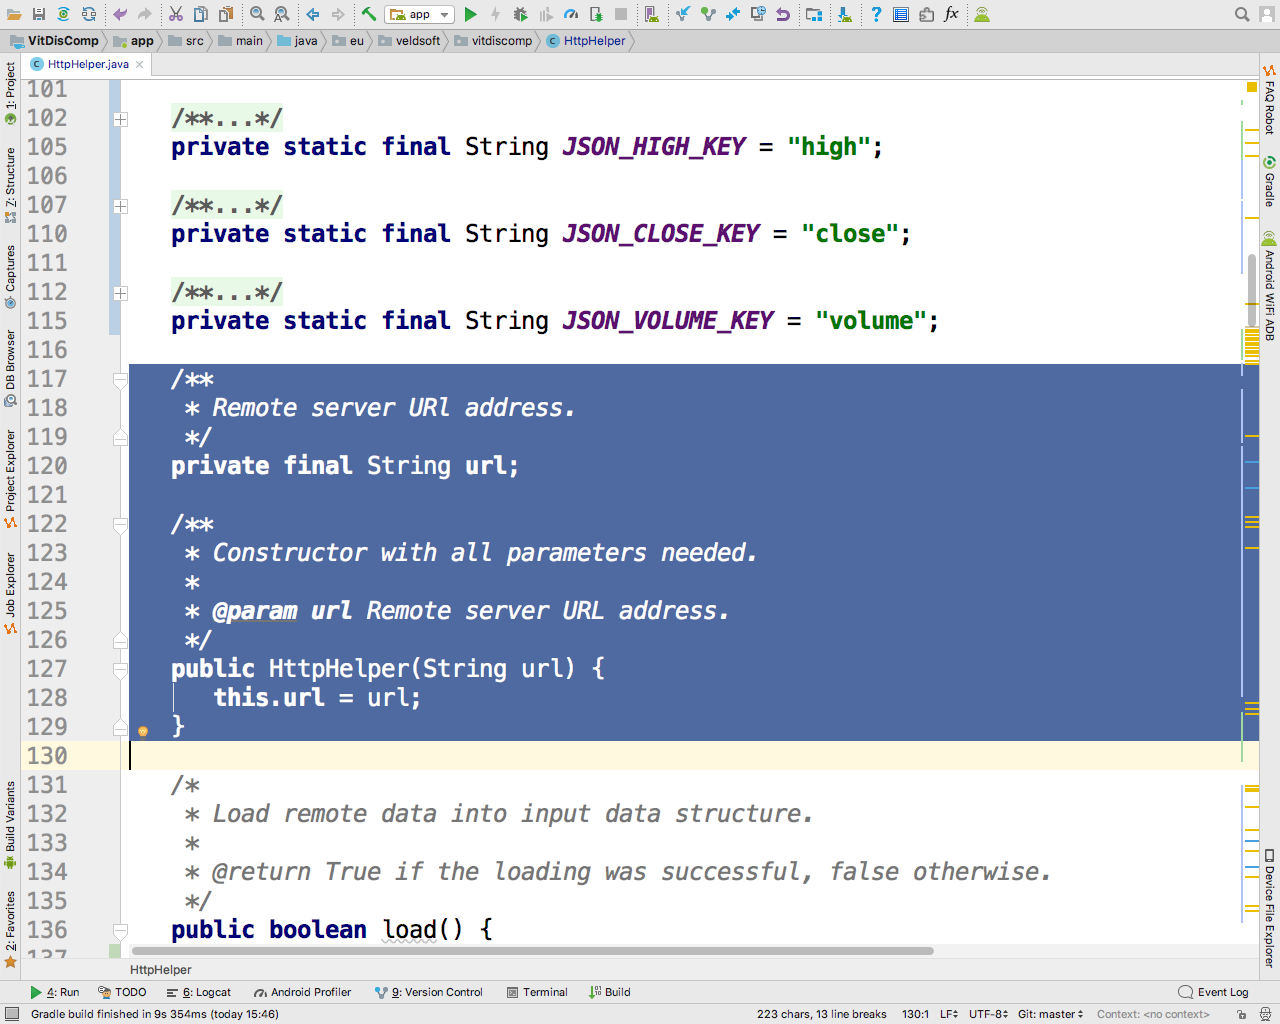
\includegraphics[height=0.45\pdfpageheight]{pic0162}
  \caption{Констркутор на спомагателния клас}
\label{fig:pic0162}
\end{figure}
\FloatBarrier

Тъй като URL адресът на отдалечения сървър е възможно да търпи многократни промени, е разумно тази информация да постъпва в конструктора на класа (Фиг. \ref{fig:pic0162}).

\begin{figure}[h]
  \centering
  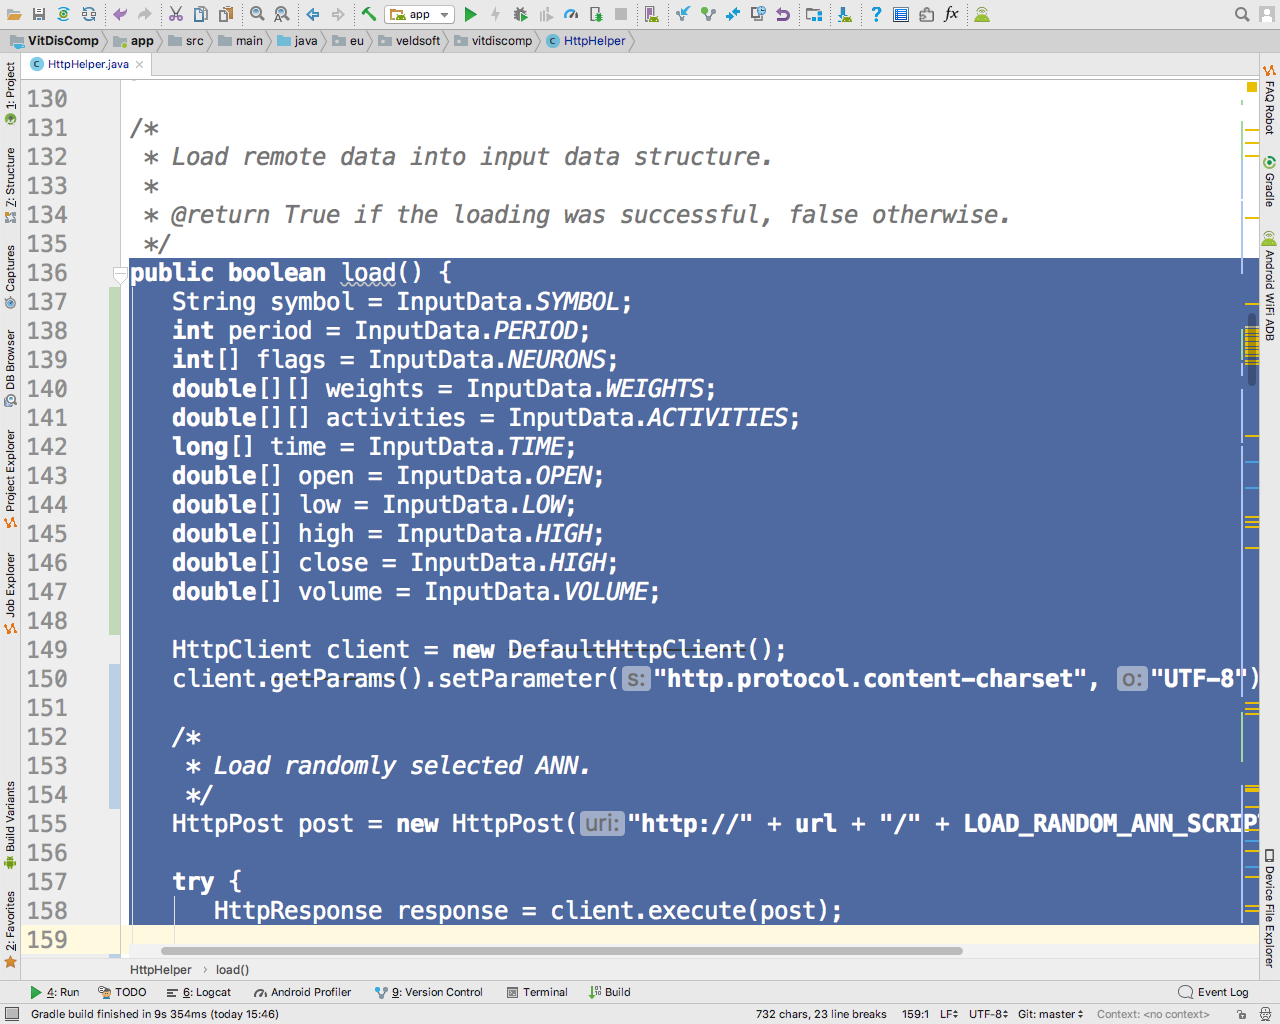
\includegraphics[height=0.45\pdfpageheight]{pic0163}
  \caption{Функция за зареждане на случайно избрана от сървъра мрежа}
\label{fig:pic0163}
\end{figure}
\FloatBarrier

За зараждане на случайно избрана мрежа се извиква определеният за целта скрипт на отдалечения сървър. Това се извършва в спомагателна функция load, която зарежда информацията в публично достъпната глобална структура за представяне на работните данни (Фиг. \ref{fig:pic0163}). 

\begin{figure}[h]
  \centering
  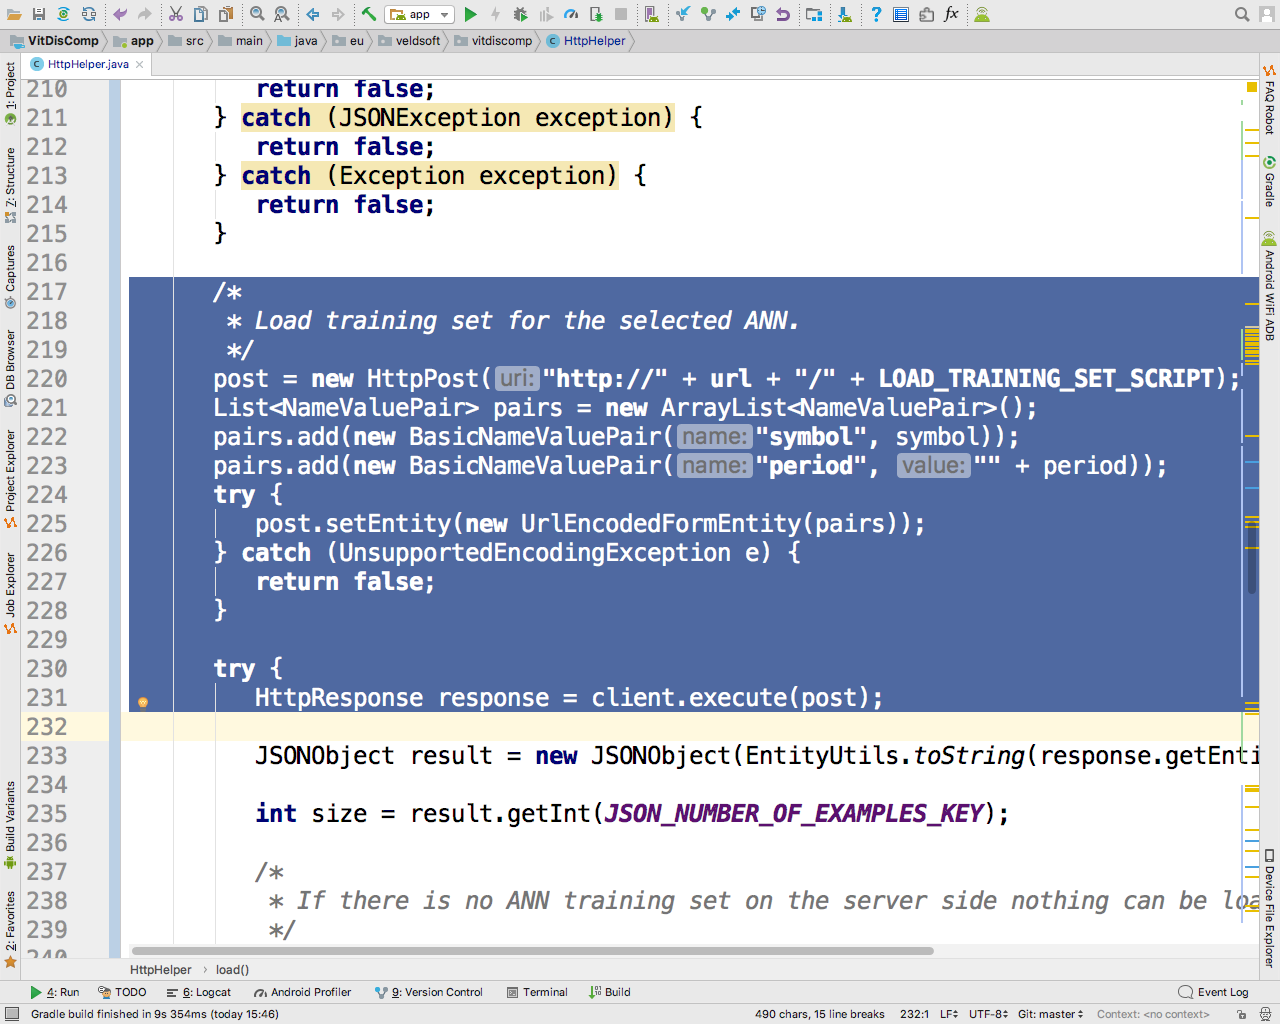
\includegraphics[height=0.45\pdfpageheight]{pic0167}
  \caption{Зареждане на тренировъчно множество}
\label{fig:pic0167}
\end{figure}
\FloatBarrier

След като бъде заредена случайно избрана мрежа, се зарежда и подходящо за мрежата тренировъчно множество  (Фиг. \ref{fig:pic0167}). За съпоставка на наличните времеви редове се използва названието на символната двойка и периодът на реда. 

\begin{figure}[h]
  \centering
  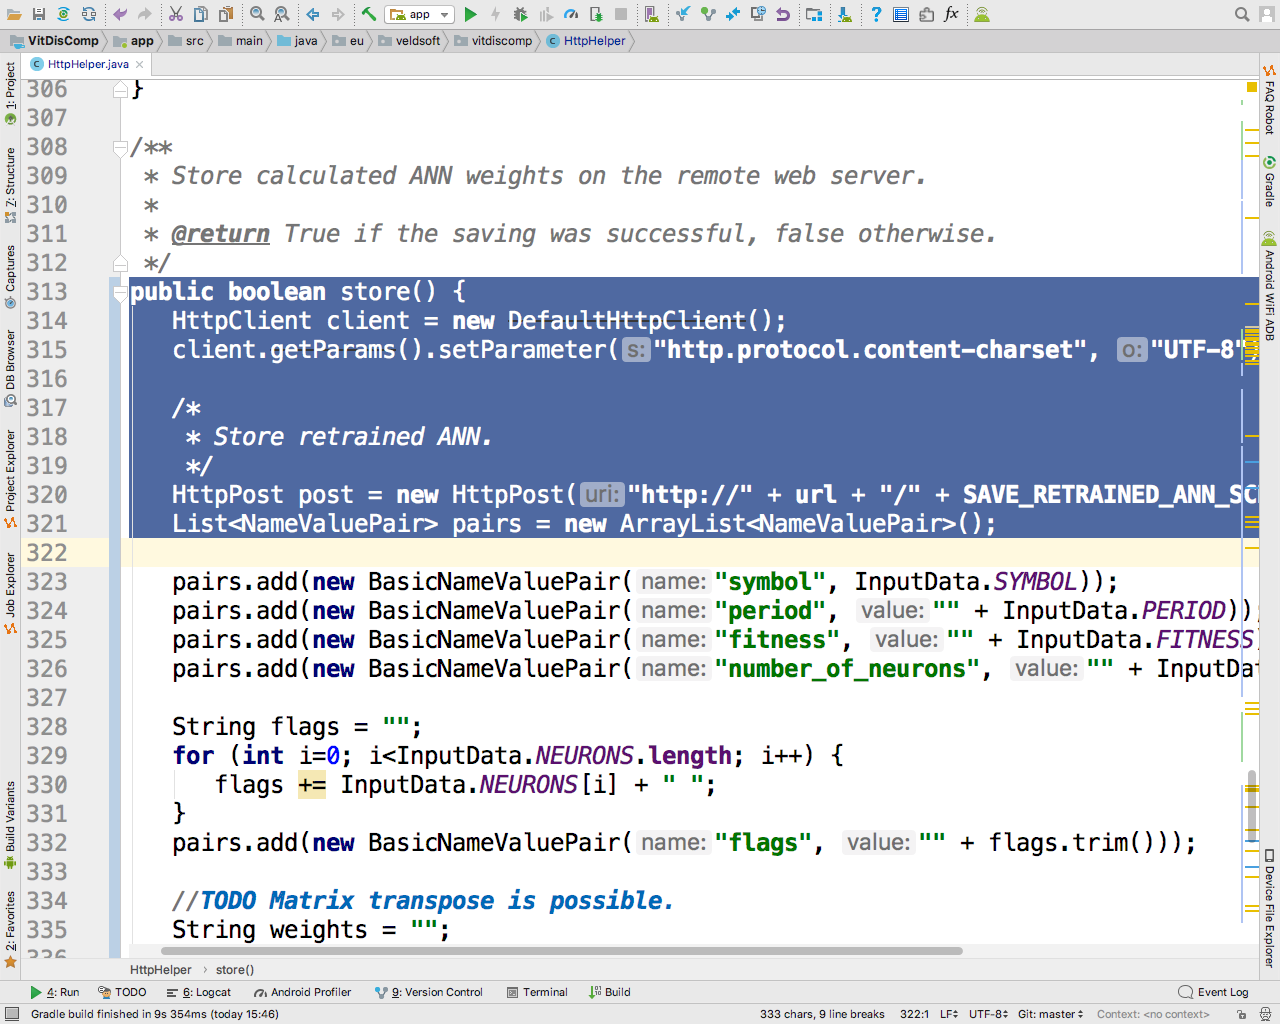
\includegraphics[height=0.45\pdfpageheight]{pic0164}
  \caption{Функция за запазване на допълнително обучавана мрежа}
\label{fig:pic0164}
\end{figure}
\FloatBarrier

При процеса за съхраняване на допълнително обучената мрежа се използва втора помощна функция save, която има за цел да изпрати по HTTP заявка информацията налична в глобалната структура с данните от обучението (Фиг. \ref{fig:pic0164}). 

\begin{figure}[h]
  \centering
  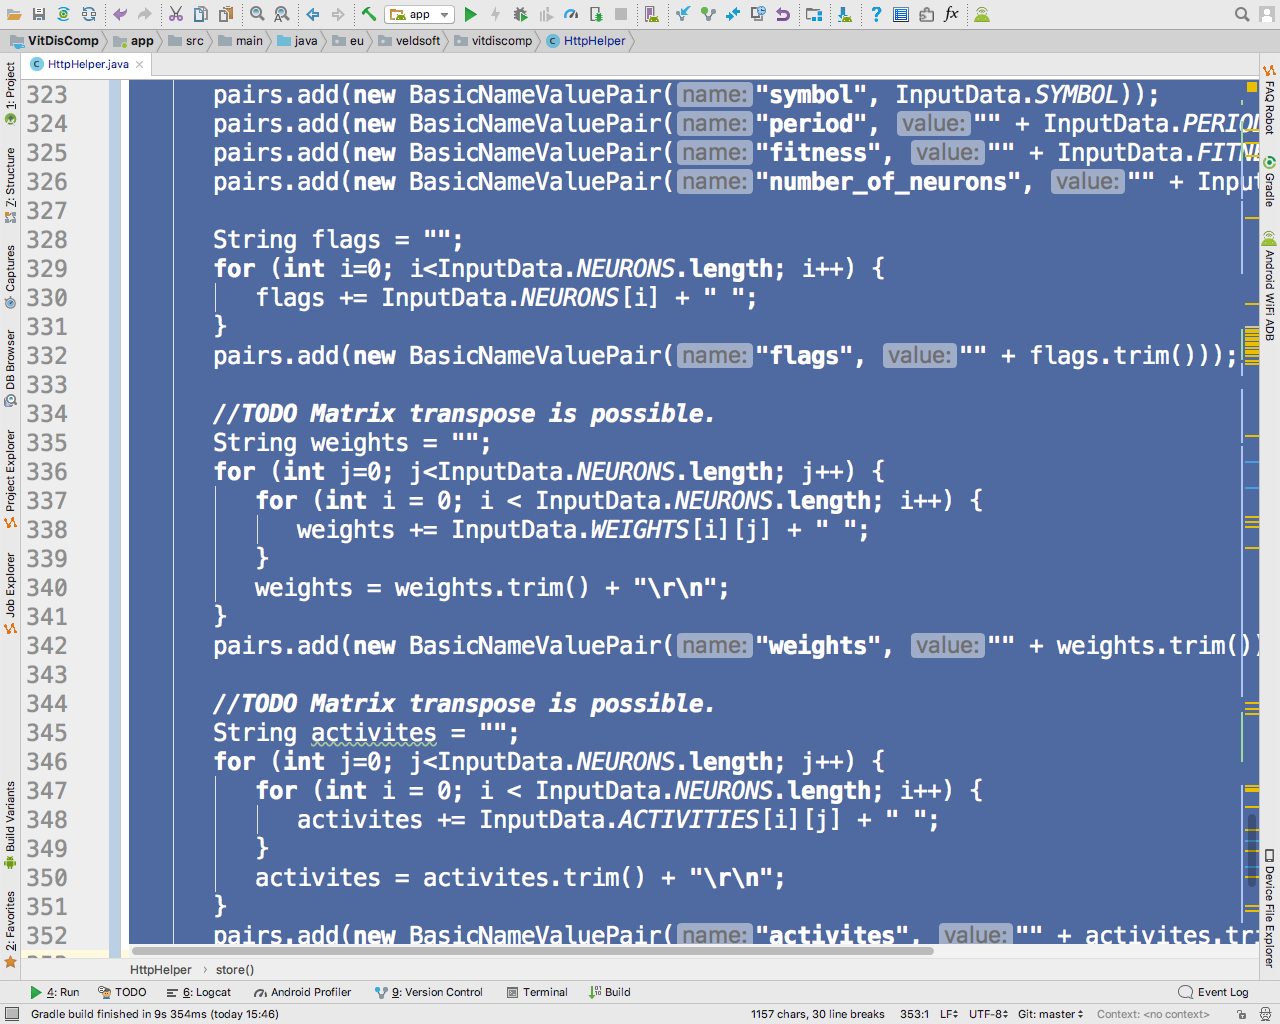
\includegraphics[height=0.45\pdfpageheight]{pic0165}
  \caption{Подготвяне на POST заявка}
\label{fig:pic0165}
\end{figure}
\FloatBarrier

Данните от глобалната структура се оформят като HTTP заявка от тип POST  като това е свързано с трансформирането им от бинарни стойности в текстови (Фиг. \ref{fig:pic0165}).

\begin{figure}[h]
  \centering
  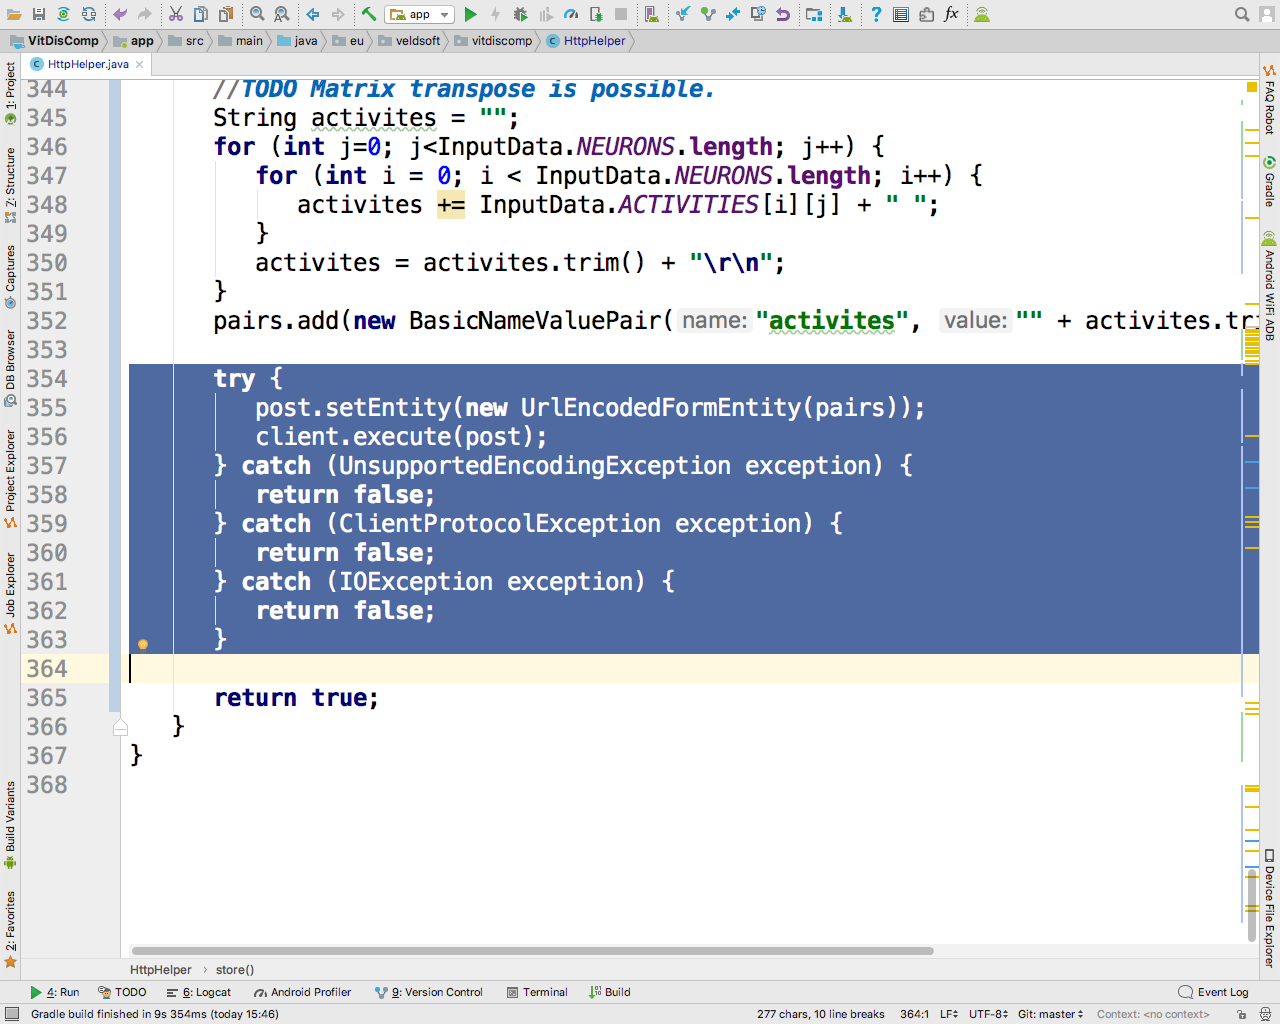
\includegraphics[height=0.45\pdfpageheight]{pic0166}
  \caption{Изпълнение на POST заявката}
\label{fig:pic0166}
\end{figure}
\FloatBarrier

Изпращането на информацията приключва с изпълнение на HTTP заявката (Фиг. \ref{fig:pic0166}).

\section{JavaScript Object Notation}

Веднъж получена по HTTP, информацията пакетирана с JSON, подлежи на синтактичен анализ и трансформиране от поток байтове във вътрешната структура за представяне на пакет за пресмятане. 

\begin{figure}[h]
  \centering
  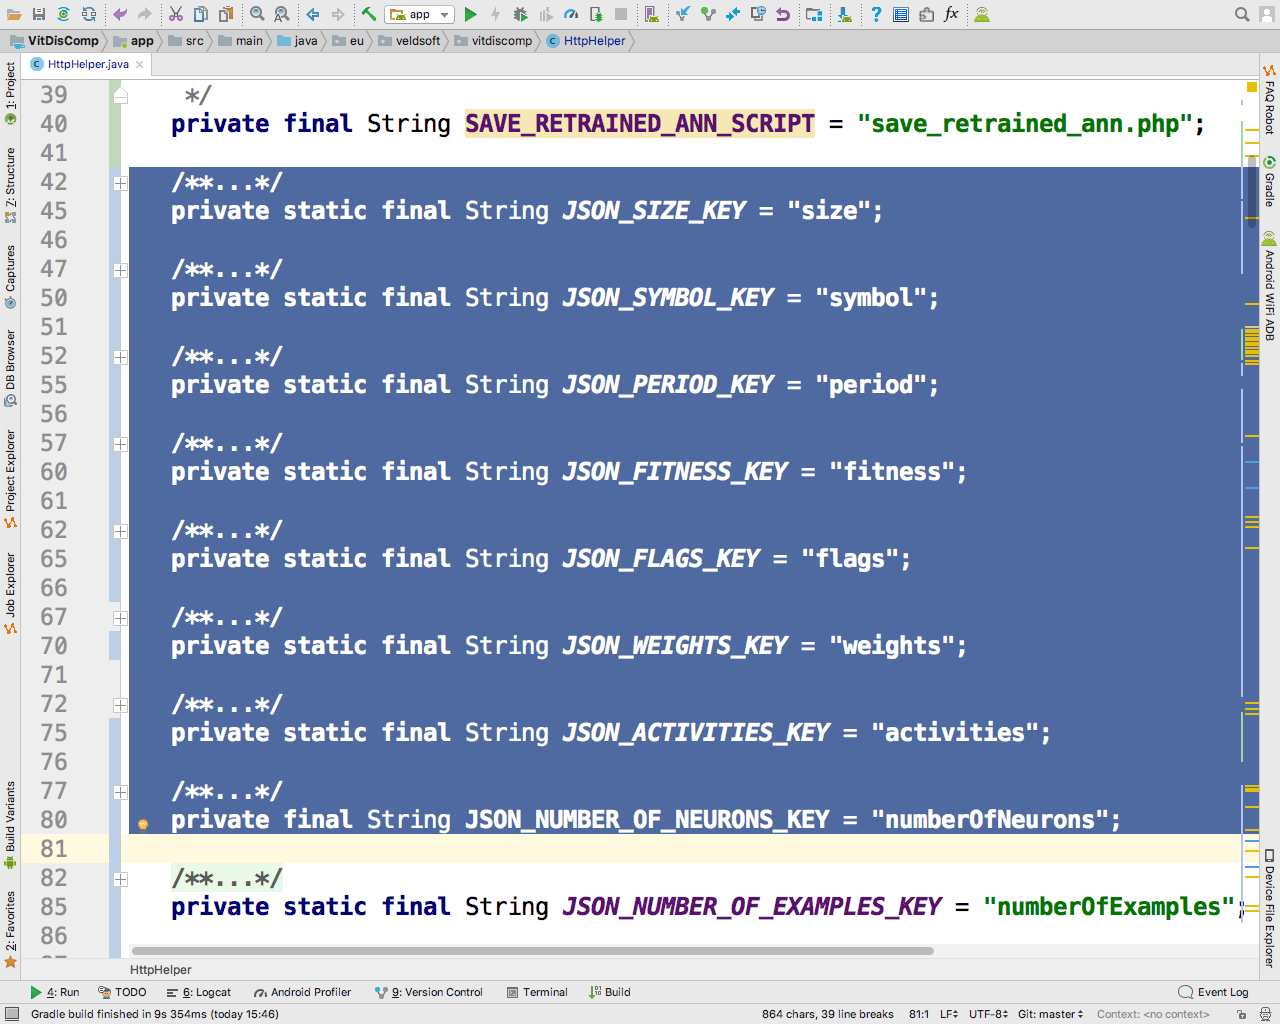
\includegraphics[height=0.45\pdfpageheight]{pic0160}
  \caption{Ключови стойности за описване на мрежата}
\label{fig:pic0160}
\end{figure}
\FloatBarrier

Една от основните роли на JSON е в изграждането на комуникационни протоколи, която в настоящата разработка се състои в информация организирана йерархично на принципа „ключ-стойност“. Тъй като комуникационните протоколи подлежат на промяна, е удачно ключовите стойности да се представят под формата на преименувани константи (Фиг. \ref{fig:pic0160},\ref{fig:pic0161}).

\begin{figure}[h]
  \centering
  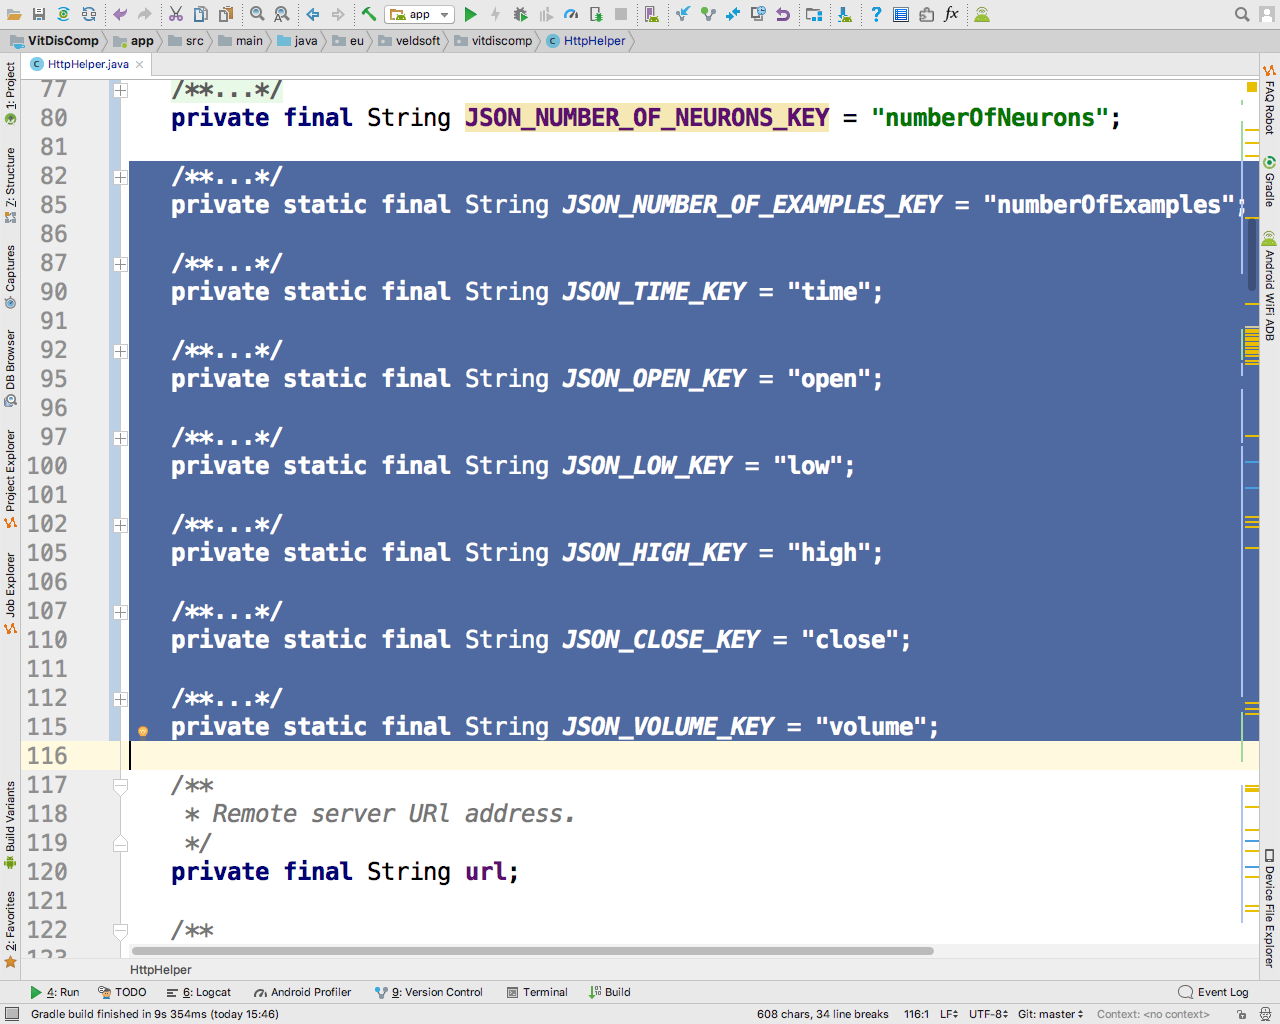
\includegraphics[height=0.45\pdfpageheight]{pic0161}
  \caption{Ключови стойности за описване на тренировъчното множество}
\label{fig:pic0161}
\end{figure}
\FloatBarrier

При зареждането на изкуствена невронна мрежа и времеви ред за обучението й от отдалечения сървър, информацията се получава с две отделни HTTP заявки. Това налага два отделни фрагмента да обработят JSON съобщенията. 

\begin{figure}[h]
  \centering
  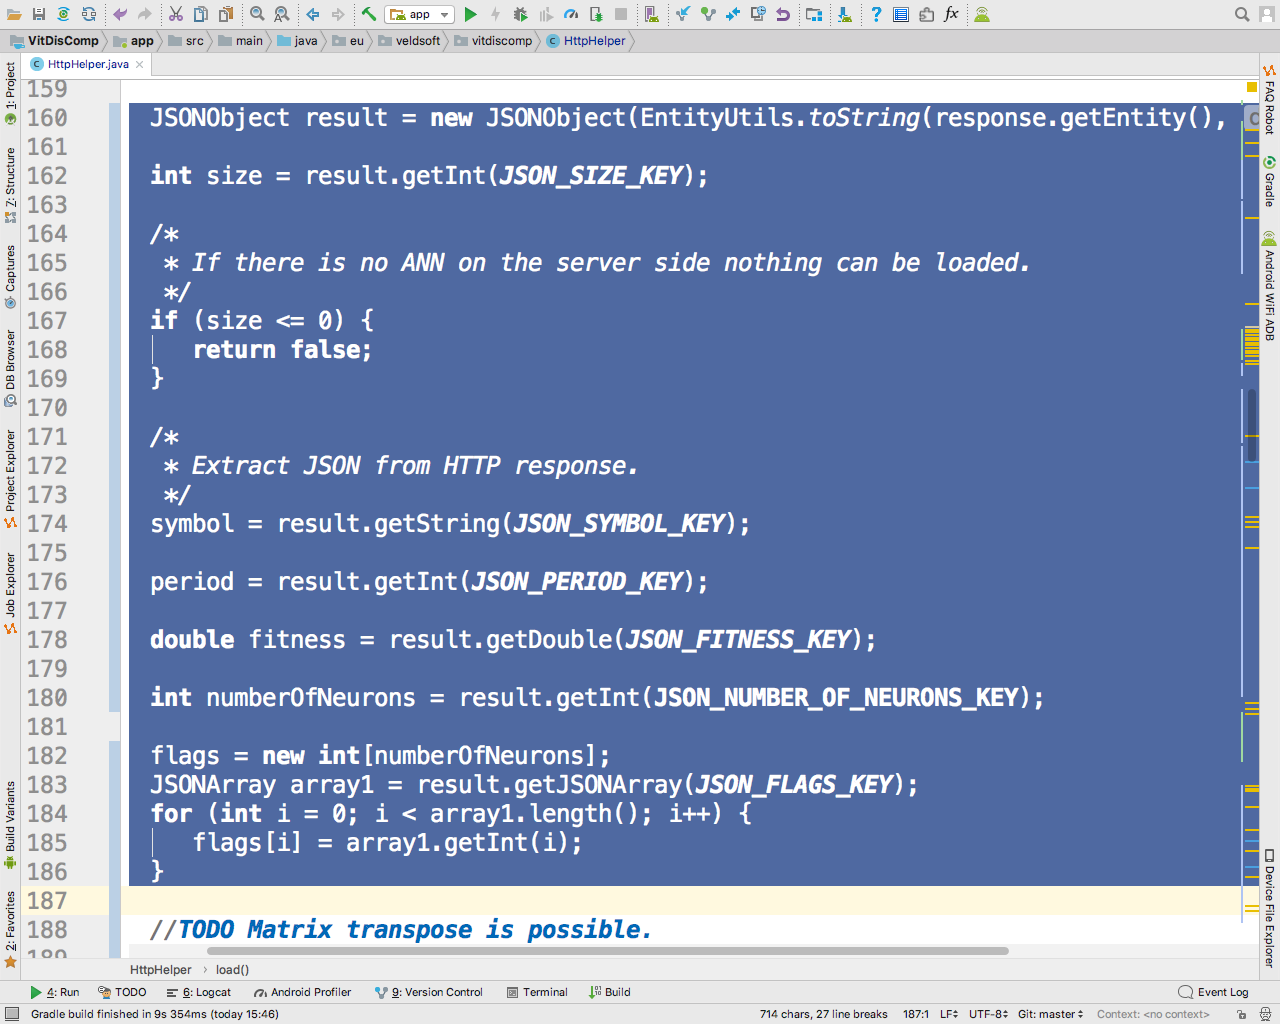
\includegraphics[height=0.45\pdfpageheight]{pic0168}
  \caption{Стойности за времевия ред и невроните}
\label{fig:pic0168}
\end{figure}
\FloatBarrier

При първия фрагмент се получава информация за вида на времевия ред, периода на времевия ред, броя неврони в мрежата и техния тип (Фиг. \ref{fig:pic0168}), стойности на теглата и стойности за силата на връзките между невроните (Фиг. \ref{fig:pic0169}).

\begin{figure}[h]
  \centering
  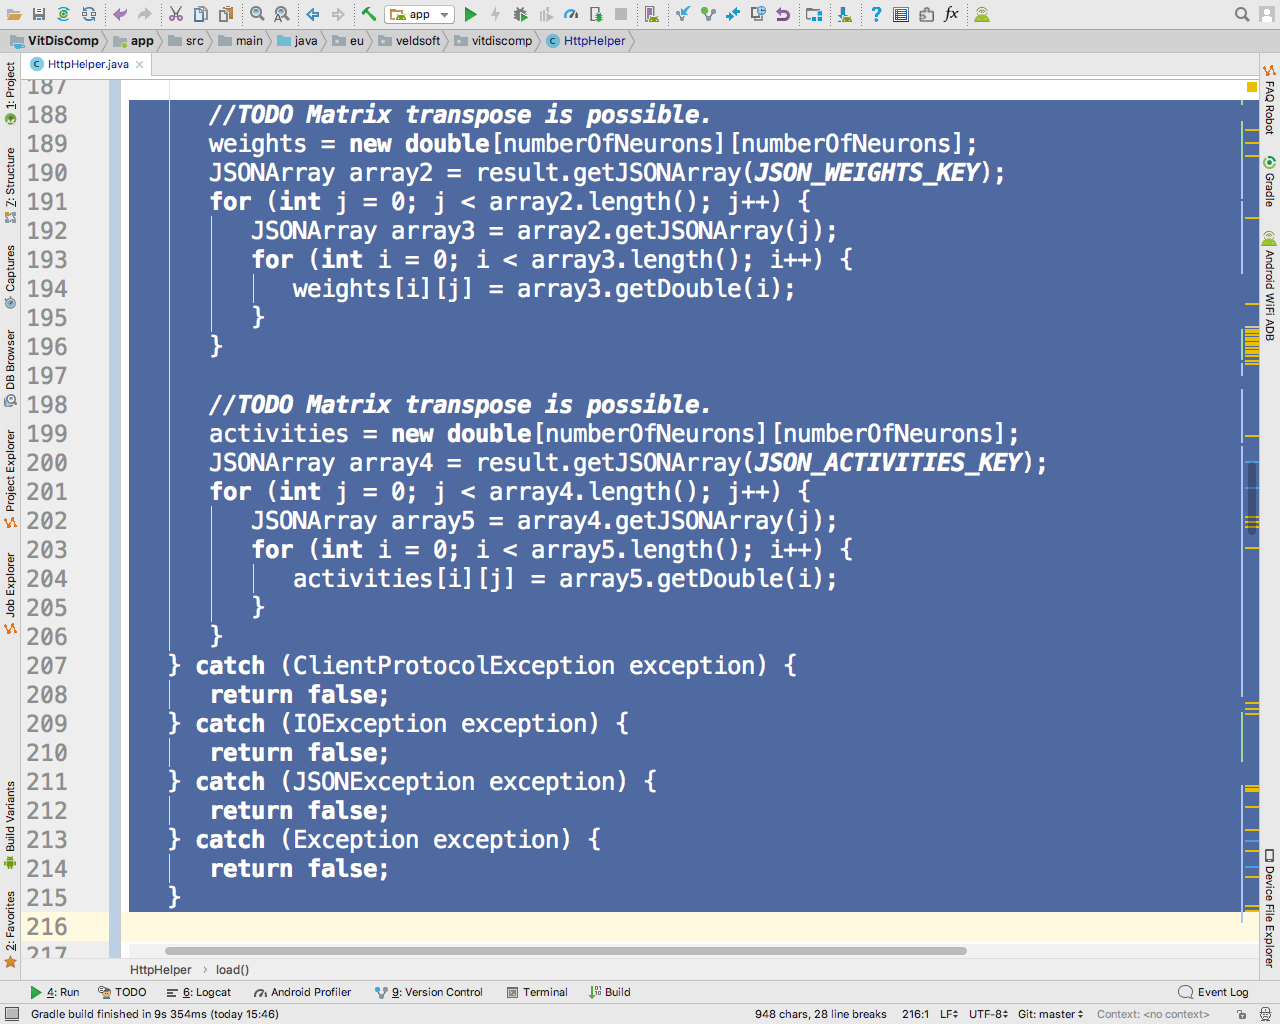
\includegraphics[height=0.45\pdfpageheight]{pic0169}
  \caption{Стойности за теглата и силата на връзките}
\label{fig:pic0169}
\end{figure}
\FloatBarrier

При втория фрагмент се получава информация за времевия ред, което включва времеви масив, масив отваря, масив най-ниска (Фиг. \ref{fig:pic0170}), масив най-висока, масив затваря и масив за търгуван обем (Фиг. \ref{fig:pic0171}).

\begin{figure}[h]
  \centering
  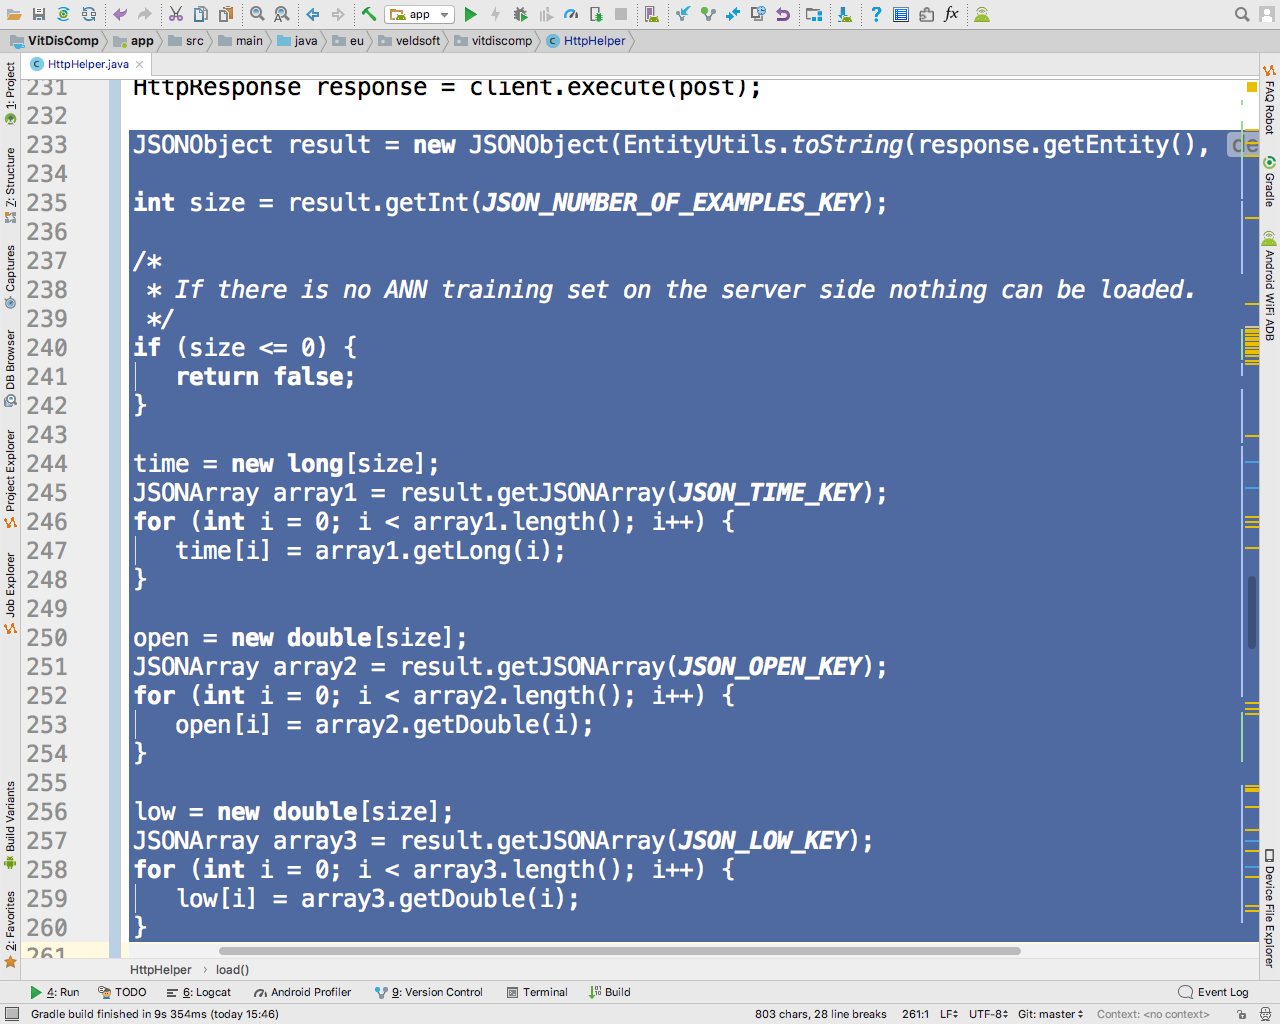
\includegraphics[height=0.45\pdfpageheight]{pic0170}
  \caption{Стойности за време, отваряне и най-ниска постигната стойност}
\label{fig:pic0170}
\end{figure}
\FloatBarrier

\begin{figure}[h]
  \centering
  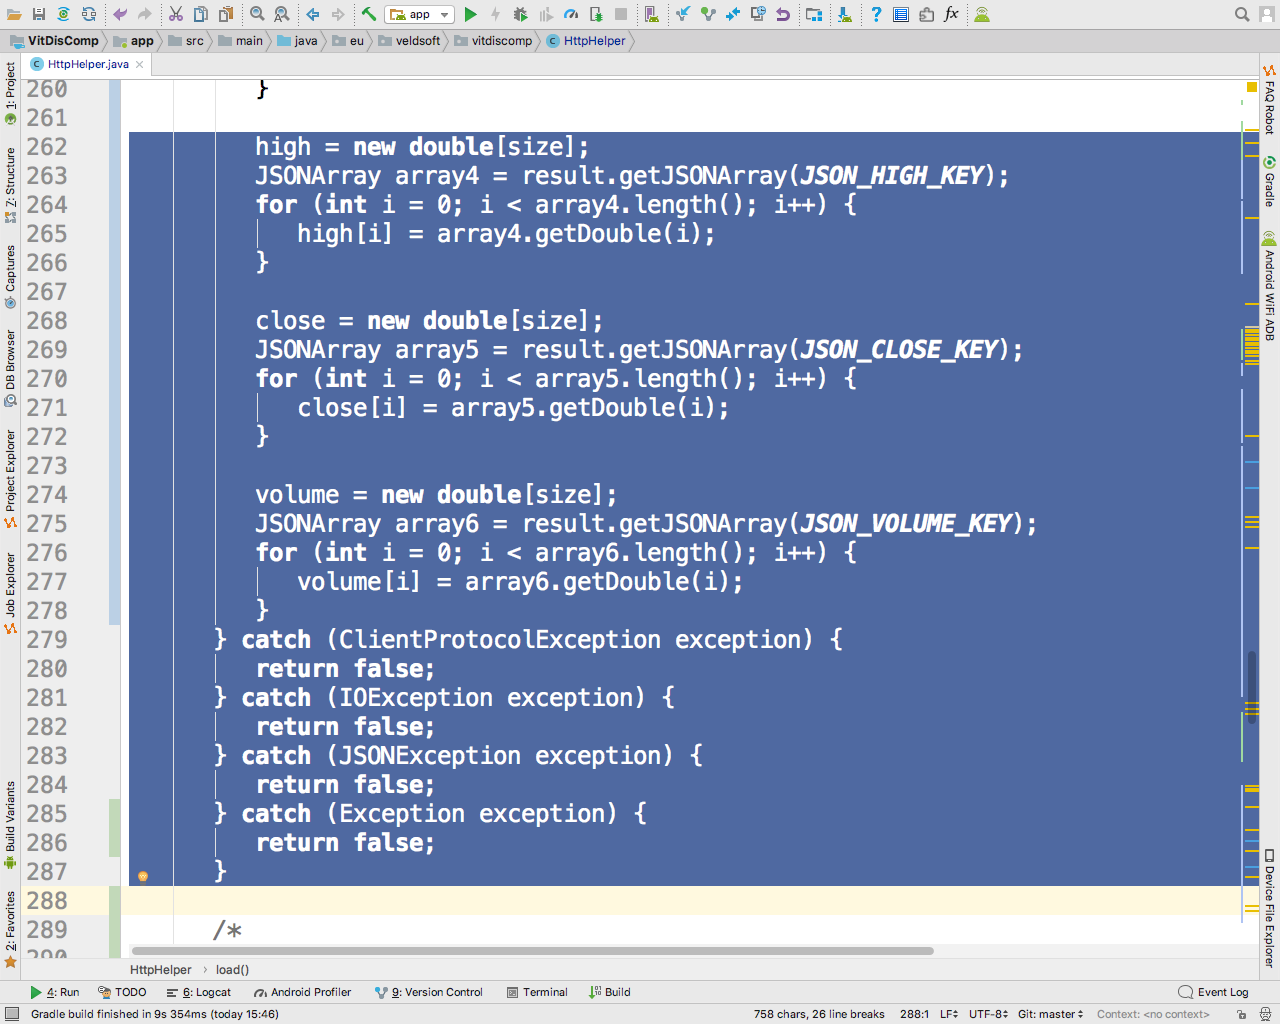
\includegraphics[height=0.45\pdfpageheight]{pic0171}
  \caption{Стойности за най-висока постигната стойност, затваряне и изтъргуван обем}
\label{fig:pic0171}
\end{figure}
\FloatBarrier

При успешно получаване на информацията от отдалечения сървър, данните се записват в глобалната структура за пресмятане (Фиг. \ref{fig:pic0172}).

\begin{figure}[h]
  \centering
  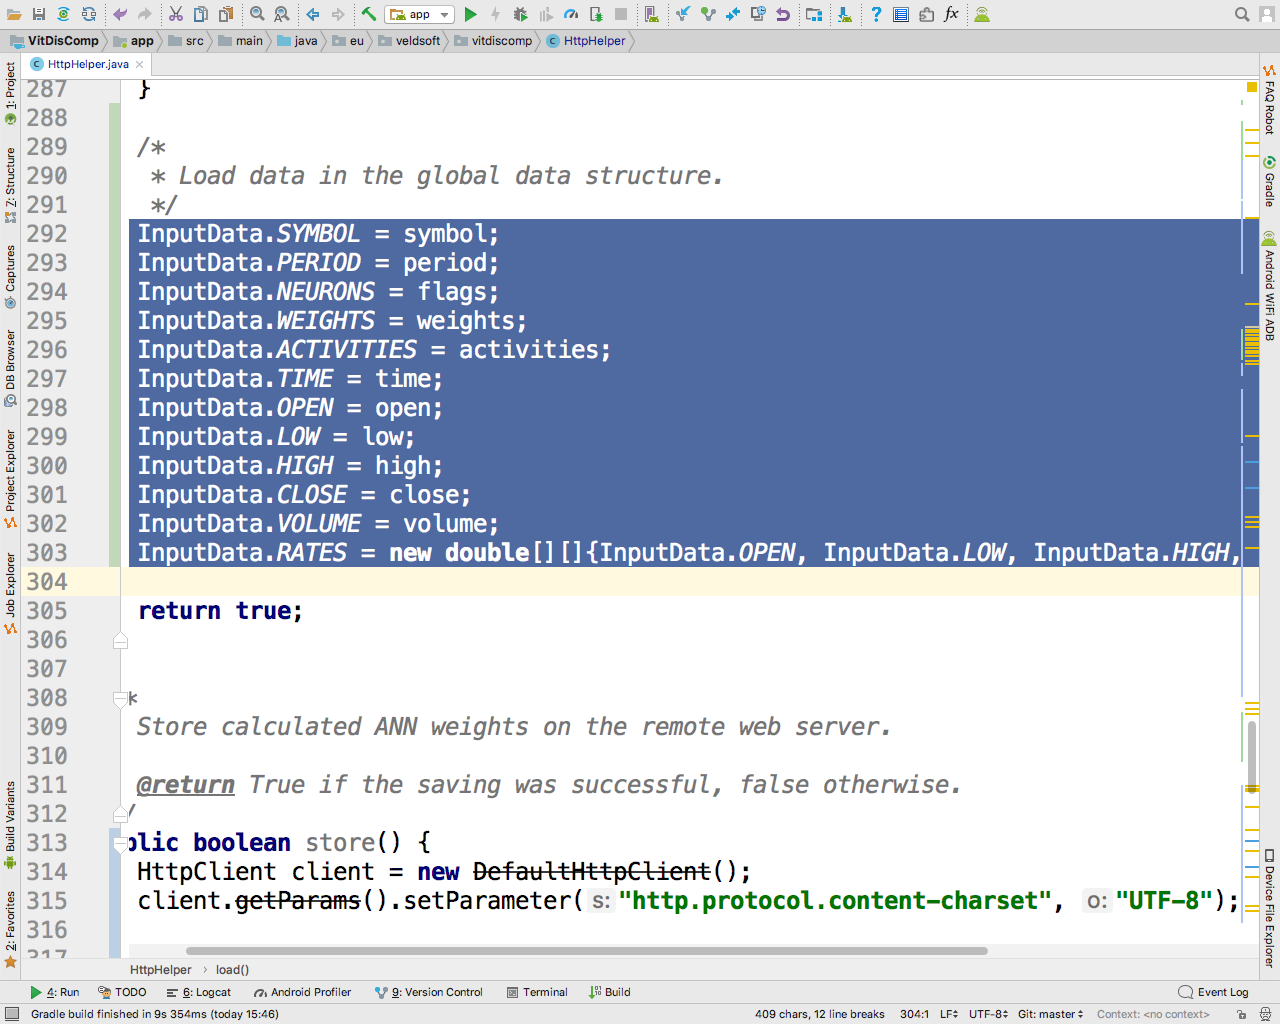
\includegraphics[height=0.45\pdfpageheight]{pic0172}
  \caption{Записване на данните в глобалната структура}
\label{fig:pic0172}
\end{figure}
\FloatBarrier
